\begin{frame}{Requirements of [RHS95] approach}
  \begin{itemize}
    \item The abstract lattice $L = 2^D$, where $D$ is a finite set
    \item Transfer functions are distributive (approach is undefined for non-distributive functions)
    \item Join (in the $L$ lattice) is union or intersection.
    \begin{itemize}
      \item Paper focuses on union problems. Every intersection problem has a complement problem whose join is union.
    \end{itemize}
    \item Examples of IFDS problem that is not a gen/kill problem: Possibly uninitialized variables, copy-constant propagation, truly live variables (backward analysis).
    \item The RHS algorithm computes JVP for IFDS frameworks.
  \end{itemize}
\end{frame}

\subsection{Dataflow functions}
\begin{frame}{Representing dataflow functions}
  \begin{block}{Definition 3.1.}
    The \emph{representation relation} of $f$, $R_f \subseteq (D \cup \{\mathbf{0}\}) \times (D \cup \{\mathbf{0}\})$, is a binary relation (i.e., graph) defined as follows:
    $$R_f =_{\text{df}} \left\{ \begin{array}{l}
      \{(\mathbf{0}, \mathbf{0})\} \\
      \cup \{(\mathbf{0}, y) \mid y \in f(\emptyset)\} \\
      \cup \{(x, y) \mid y \in f(\{x\}) \text{ and } y \notin f(\emptyset)\}
    \end{array}\right. \quad \square$$
  \end{block}

  \vspace{0.5em}
  Representation relation can be thought of as a \emph{Graph} with $2(D + 1)$ nodes.
\end{frame}

\begin{frame}{Representing dataflow functions}
  \begin{block}{Definition 3.1.}
    The \emph{representation relation} of $f$, $R_f \subseteq (D \cup \{\mathbf{0}\}) \times (D \cup \{\mathbf{0}\})$, is a binary relation (i.e., graph) defined as follows:
    $$R_f =_{\text{df}} \left\{ \begin{array}{l}
      \{(\mathbf{0}, \mathbf{0})\} \\
      \cup \{(\mathbf{0}, y) \mid y \in f(\emptyset)\} \\
      \cup \{(x, y) \mid y \in f(\{x\}) \text{ and } y \notin f(\emptyset)\}
    \end{array}\right. \quad \square$$
  \end{block}

  \vspace{0.2em}
  \noindent
  \begin{minipage}[c]{0.45\textwidth}
    \onslide<1>{%
      Identity function\\
      \(f = \lambda S.S\)\\
    }
    \onslide<2>{%
      Constant function\\
      \(f = \lambda S.\{b\}\)
    }
  \end{minipage}
  \hfill
  \begin{minipage}[c]{0.5\textwidth}
  \centering
    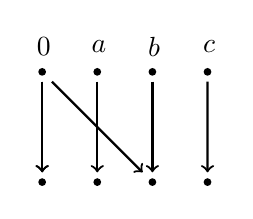
\begin{tikzpicture}[scale=0.7]
      \node  at (0.03,2.46) {$0$};
      \node  at (1.03,2.46) {$a$};
      \node  at (2.03,2.46) {$b$};
      \node  at (3.03,2.46) {$c$};

      \node (0) at (0,2) {};
      \node (a) at (1,2) {};
      \node (b) at (2,2) {};
      \node (c) at (3,2) {};

      \fill (0) circle (2pt);
      \fill (a) circle (2pt);
      \fill (b) circle (2pt);
      \fill (c) circle (2pt);

      \node (0b) at (0,0) {};
      \node (ab) at (1,0) {};
      \node (bb) at (2,0) {};
      \node (cb) at (3,0) {};

      \fill (0b) circle (2pt);
      \fill (ab) circle (2pt);
      \fill (bb) circle (2pt);
      \fill (cb) circle (2pt);

      \onslide<1>{\draw[->, thick] (0) -- (0b);}
      \onslide<1>{\draw[->, thick] (a) -- (ab);}
      \onslide<1>{\draw[->, thick] (b) -- (bb);}
      \onslide<1>{\draw[->, thick] (c) -- (cb);}
      \onslide<2>{\draw[->, thick] (0) -- (0b);}
      \onslide<2>{\draw[->, thick] (0) -- (bb);}
    \end{tikzpicture}
  \end{minipage}

  \vspace{0.5em}
  \hfill {\tiny (Credit: Prof. Reps)}
\end{frame}

\begin{frame}{Representing dataflow functions - Exercise 1}
  Try constructing the representation relation without the definition

  \vspace{0.5em}
  \begin{minipage}{0.48\textwidth}
    $$f = \lambda S.(S - \{b\}) \cup \{c\}$$
  \end{minipage}
  \onslide<2>{
  \begin{minipage}{0.48\textwidth}
    \centering
    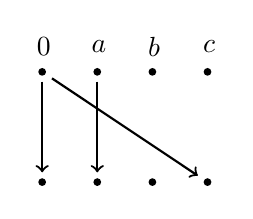
\begin{tikzpicture}[scale=0.7]
      \node  at (0.03,2.46) {$0$};
      \node  at (1.03,2.46) {$a$};
      \node  at (2.03,2.46) {$b$};
      \node  at (3.03,2.46) {$c$};

      \node (0) at (0,2) {};
      \node (a) at (1,2) {};
      \node (b) at (2,2) {};
      \node (c) at (3,2) {};

      \fill (0) circle (2pt);
      \fill (a) circle (2pt);
      \fill (b) circle (2pt);
      \fill (c) circle (2pt);

      \node (0b) at (0,0) {};
      \node (ab) at (1,0) {};
      \node (bb) at (2,0) {};
      \node (cb) at (3,0) {};

      \fill (0b) circle (2pt);
      \fill (ab) circle (2pt);
      \fill (bb) circle (2pt);
      \fill (cb) circle (2pt);

      \draw[->, thick] (0) -- (0b);
      \draw[->, thick] (a) -- (ab);
      \draw[->, thick] (0) -- (cb);
    \end{tikzpicture}
  \end{minipage}

  \vspace{1em}
  \hfill {\tiny (Credit: Prof. Reps)}
  }
\end{frame}

\begin{frame}{Representing dataflow functions - Exercise 2}
  \begin{minipage}{0.48\textwidth}
    \small
    $f = \lambda S. \text{if } a \in S$\\
    \quad $\text{then } S \cup \{b\}$\\
    \quad $\text{else } S - \{b\}$
  \end{minipage}
  \begin{minipage}{0.48\textwidth}
    \centering
    \onslide<2->{
    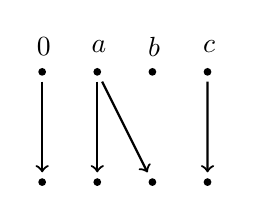
\begin{tikzpicture}[scale=0.7]
      \node  at (0.03,2.46) {$0$};
      \node  at (1.03,2.46) {$a$};
      \node  at (2.03,2.46) {$b$};
      \node  at (3.03,2.46) {$c$};

      \node (0) at (0,2) {};
      \node (a) at (1,2) {};
      \node (b) at (2,2) {};
      \node (c) at (3,2) {};

      \fill (0) circle (2pt);
      \fill (a) circle (2pt);
      \fill (b) circle (2pt);
      \fill (c) circle (2pt);

      \node (0b) at (0,0) {};
      \node (ab) at (1,0) {};
      \node (bb) at (2,0) {};
      \node (cb) at (3,0) {};

      \fill (0b) circle (2pt);
      \fill (ab) circle (2pt);
      \fill (bb) circle (2pt);
      \fill (cb) circle (2pt);

      \draw[->, thick] (0) -- (0b);
      \draw[->, thick] (a) -- (ab);
      \draw[->, thick] (a) -- (bb);
      \draw[->, thick] (c) -- (cb);
    \end{tikzpicture}}
  \end{minipage}

  \vspace{1em}
  \begin{minipage}{0.48\textwidth}
    \small
    $f = \lambda S. \text{if } a \in S \text{ OR } b \in S$\\
    \quad $\text{then } S \cup \{c\}$\\
    \quad $\text{else } S - \{c\}$
  \end{minipage}
  \begin{minipage}{0.48\textwidth}
    \centering
    \onslide<2>{
    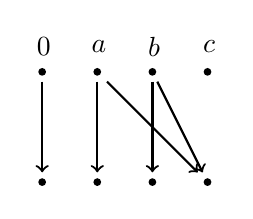
\begin{tikzpicture}[scale=0.7]
      \node  at (0.03,2.46) {$0$};
      \node  at (1.03,2.46) {$a$};
      \node  at (2.03,2.46) {$b$};
      \node  at (3.03,2.46) {$c$};

      \node (0) at (0,2) {};
      \node (a) at (1,2) {};
      \node (b) at (2,2) {};
      \node (c) at (3,2) {};

      \fill (0) circle (2pt);
      \fill (a) circle (2pt);
      \fill (b) circle (2pt);
      \fill (c) circle (2pt);

      \node (0b) at (0,0) {};
      \node (ab) at (1,0) {};
      \node (bb) at (2,0) {};
      \node (cb) at (3,0) {};

      \fill (0b) circle (2pt);
      \fill (ab) circle (2pt);
      \fill (bb) circle (2pt);
      \fill (cb) circle (2pt);

      \draw[->, thick] (0) -- (0b);
      \draw[->, thick] (a) -- (ab);
      \draw[->, thick] (a) -- (cb);
      \draw[->, thick] (b) -- (bb);
      \draw[->, thick] (b) -- (cb);
    \end{tikzpicture}
    }
  \end{minipage}
\end{frame}

